\documentclass[a4paper]{article}
\usepackage{mathtext}
\usepackage[russian]{babel}
\usepackage{indentfirst}
\usepackage[pdftex]{graphicx}
\usepackage{multirow}
\usepackage{csvsimple}
\usepackage[left=2cm,right=2cm,top=2cm,bottom=2cm]{geometry}
% Название работы здесь
\title{Работа 1.3.3 Определение вязкости воздуха по скорости течения через тонкие трубки}
\author{Иван Сладков}
\begin{document}
\maketitle
\section{Аннотация}
% Текст аннотации пиши здесь
В данной работе проводится экспериментальное выявление участка сформировавшегося ламинарного течения; экспериментально определяются режимы ламинарного и турбулентного течения; проводится определение числа Рейнольдса.
\section{Теоретические сведения}
% Теоретические сведения
Характер движения газа по трубке определяется числом Рейнольдса:
\begin{equation}
Re = \frac{v r \rho}{\eta},
\label{eq:Re}
\end{equation}
где $v$ - скорость потока, $r$ - радиус трубки, $\rho$ - плотность жидкости, $\eta$ - вязкость. Переход от ламинарного движения к турбулентному: $Re \sim 1000$.

Для ламинарного течения при постоянном удельном объёме верна формула Пуазейля:
\begin{equation}
Q_V = \frac{\pi r^4}{8 l \eta}(P_1 - P_2),
\label{eq:Pu}
\end{equation}
где $P_1 - P_2$ - разность давлений в двух сечениях, расстояние между которыми - $l$. Формула позволяет определить вязкость по расходу $Q_V$.

Ламинарное течение газа устанавливается на расстоянии
\begin{equation}
a \sim 0.2 r * Re.
\label{eq:Aa}
\end{equation}
Градиент давления на участке с турбулентным течением больше, чем на участке с ламинарным, что позволяет разделить их экспериментально.
\section{Оборудование и инструментальные погрешности}
% Оборудование и инструментальные погрешности

%{\bf Прибор1: } $\Delta = \pm 1 $ мм
{\bf Газовый счётчик: } $\Delta = \pm 0.1 $ л

{\bf Микроманометр: } $\Delta = \pm 1*10^{-5} $ Па

{\bf Секундомер: } $\Delta = \pm 0.1 $ с

Установка, использованная в опыте, изображена на рисунке \ref{fig:De}.
\begin{figure}[htbp]
	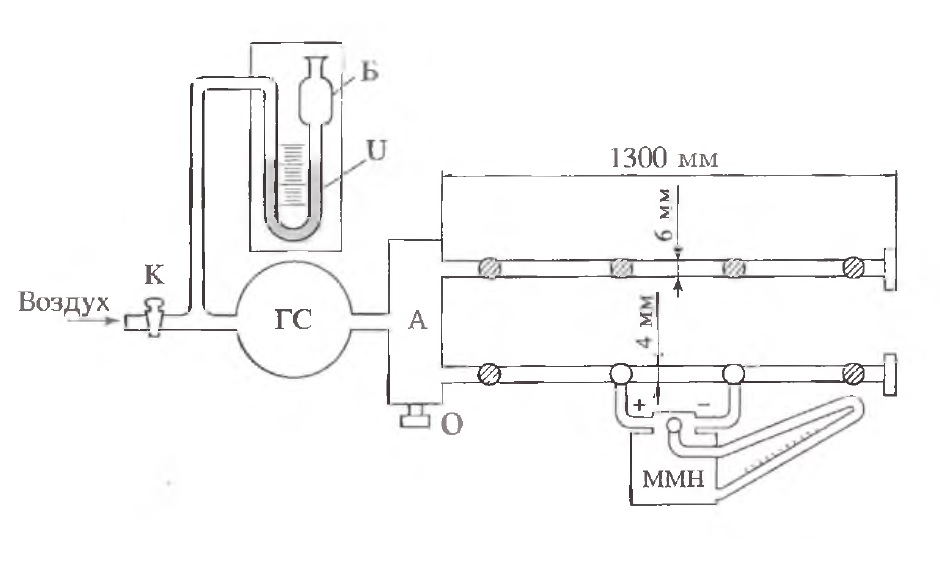
\includegraphics[scale=0.5]{1.jpg}
	\caption{Установка для определения вязкости воздуха}
	\label{fig:De}
\end{figure}

\section{Результаты измерений и обработка данных}
\subsection{Подготовка к опыту}
По формуле \ref{eq:Aa} определим расстояние при $Re = 1000$:
\begin{table}[htbp]
	\centering
		\begin{tabular}{|l|l|lll}
\cline{1-2}
\textbf{Радиус трубки, см} & \textbf{Длина уст. потока, см} &  &  &  \\ \cline{1-2}
0.29                       & 58                             &  &  &  \\ \cline{1-2}
0.15                       & 30                             &  &  &  \\ \cline{1-2}
0.205                      & 41                             &  &  &  \\ \cline{1-2}
\end{tabular}
	\caption{Длина установления ламинарного потока}
	\label{tab:Le}
\end{table}
\subsection{Измерение вязкости воздуха}
Зависимость $\Delta P(Q)$ выражается в виде таблицы \ref{tab:Dp} и графика \ref{fig:Dp}.
\begin{table}[htbp]
	\centering
	\begin{tabular}{lllll}
\cline{1-3}
\multicolumn{1}{|l|}{Радиус трубки, см}      & \multicolumn{1}{l|}{Расход, $см^3/с$} & \multicolumn{1}{l|}{Разность давлений, Б} &  &  \\ \cline{1-3}
\multicolumn{1}{|l|}{\multirow{5}{*}{0.205}} & \multicolumn{1}{l|}{159}          & \multicolumn{1}{l|}{4.35E+03}             &  &  \\ \cline{2-3}
\multicolumn{1}{|l|}{}                       & \multicolumn{1}{l|}{141}          & \multicolumn{1}{l|}{3.47E+03}             &  &  \\ \cline{2-3}
\multicolumn{1}{|l|}{}                       & \multicolumn{1}{l|}{121}          & \multicolumn{1}{l|}{2.57E+03}             &  &  \\ \cline{2-3}
\multicolumn{1}{|l|}{}                       & \multicolumn{1}{l|}{103}          & \multicolumn{1}{l|}{1.71E+03}             &  &  \\ \cline{2-3}
\multicolumn{1}{|l|}{}                       & \multicolumn{1}{l|}{66.2}         & \multicolumn{1}{l|}{922}                  &  &  \\ \cline{1-3}
\multicolumn{1}{|l|}{\multirow{5}{*}{0.29}}  & \multicolumn{1}{l|}{301}          & \multicolumn{1}{l|}{2.71E+03}             &  &  \\ \cline{2-3}
\multicolumn{1}{|l|}{}                       & \multicolumn{1}{l|}{253}          & \multicolumn{1}{l|}{1.98E+03}             &  &  \\ \cline{2-3}
\multicolumn{1}{|l|}{}                       & \multicolumn{1}{l|}{207}          & \multicolumn{1}{l|}{1.39E+03}             &  &  \\ \cline{2-3}
\multicolumn{1}{|l|}{}                       & \multicolumn{1}{l|}{150}          & \multicolumn{1}{l|}{628}                  &  &  \\ \cline{2-3}
\multicolumn{1}{|l|}{}                       & \multicolumn{1}{l|}{124}          & \multicolumn{1}{l|}{333}                  &  &  \\ \cline{1-3}
\end{tabular}
	\caption{Зависимость разности давлений от расхода}
	\label{tab:Dp}
\end{table}
\begin{figure}[htbp]
		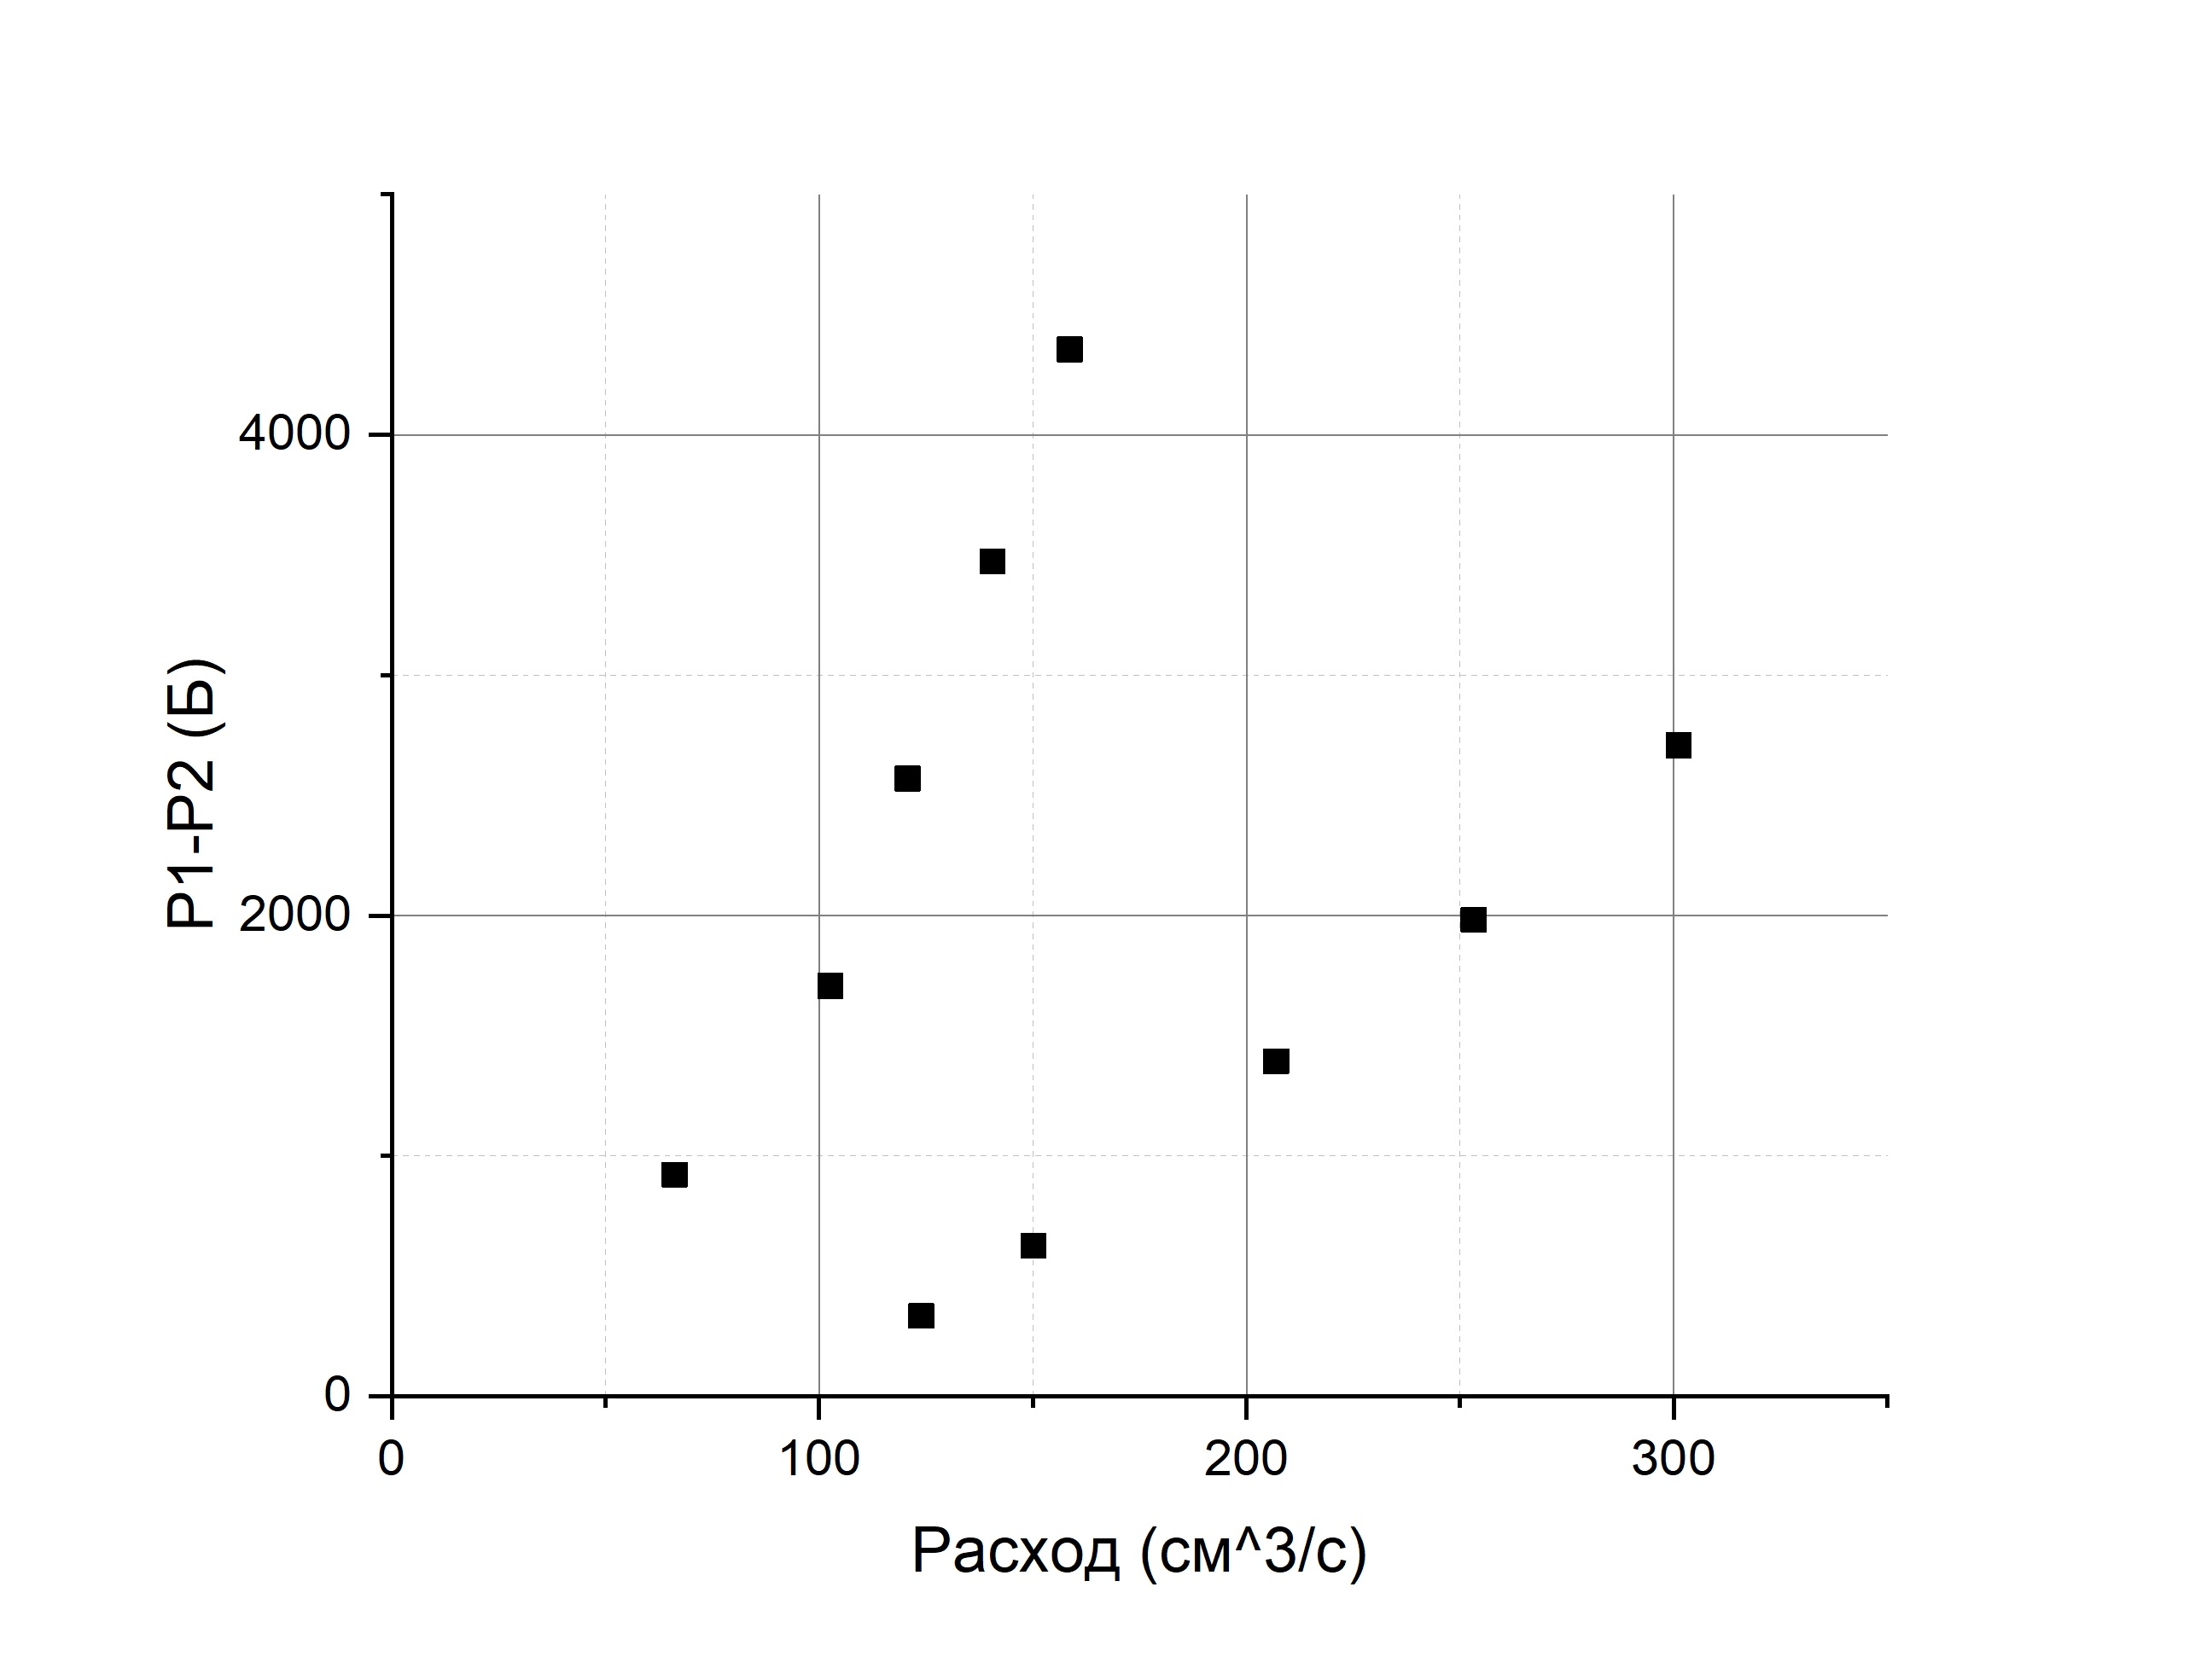
\includegraphics[scale=0.25]{2.jpg}
	\caption{График зависимости разности давлений от расхода}
	\label{fig:Dp}
\end{figure}

\subsubsection{Расчёт чисел Рейнольдса}

Оценим числа Рейнольдса для всех опытов. В формуле \ref{eq:Re} возьмём табличное значение вязкости: $18*10^{-5}$ пуаз.

% Please add the following required packages to your document preamble:
% \usepackage{multirow}
\begin{table}[htbp]
\centering
\begin{tabular}{|l|l|l|}
\hline
Радиус трубки, см      & № опыта & Число Рейнольдса \\ \hline
\multirow{5}{*}{0.205} & 1       & 1649             \\ \cline{2-3} 
                       & 2       & 1462             \\ \cline{2-3} 
                       & 3       & 1255             \\ \cline{2-3} 
                       & 4       & 1067             \\ \cline{2-3} 
                       & 5       & 687.7            \\ \hline
\multirow{5}{*}{0.290} & 1       & 2213             \\ \cline{2-3} 
                       & 2       & 1860             \\ \cline{2-3} 
                       & 3       & 1521             \\ \cline{2-3} 
                       & 4       & 1103             \\ \cline{2-3} 
                       & 5       & 910.2            \\ \hline
\end{tabular}
\label{tab:Re}
\caption{Числа Рейнольдса в разных опытах}
\end{table}

Из таблицы \ref{tab:Re} и графика \ref{fig:Dp} видно, что ламинарность течения не достигнута. Попытаемся определить вязкость по небольшому линейному участку графика. См. рисунок 
\ref{fig:4} .
\begin{figure}
	\centering
		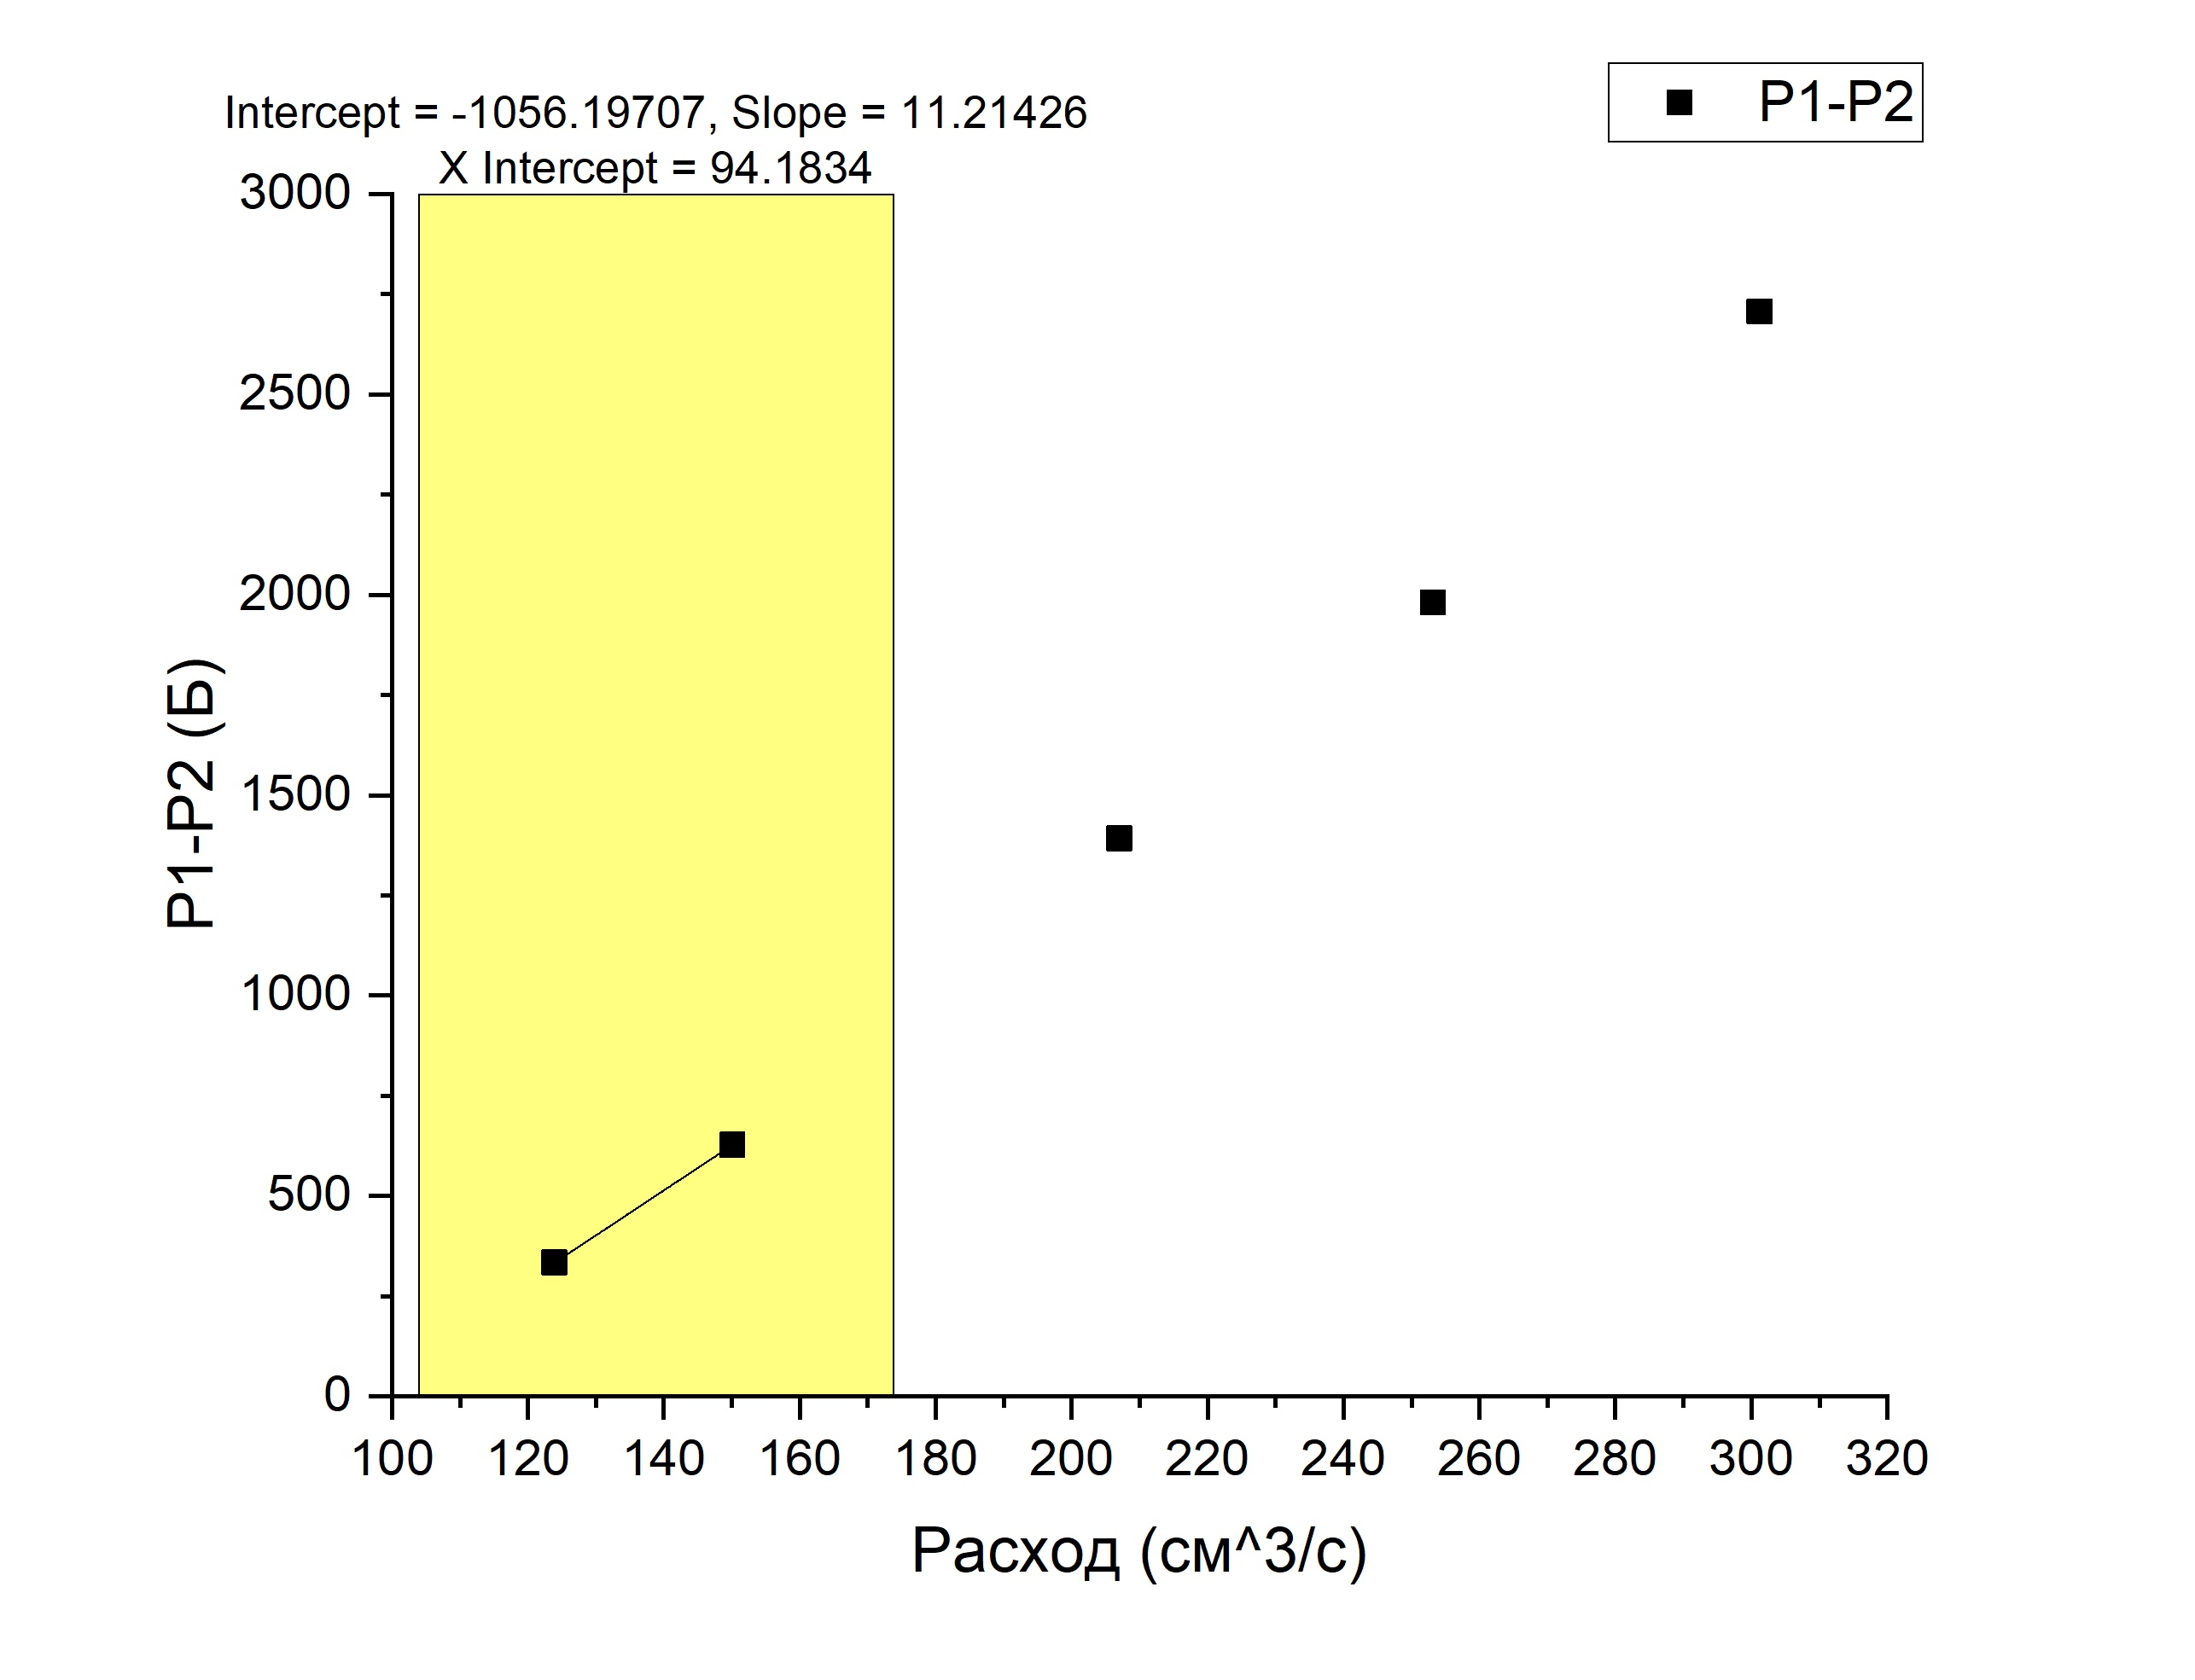
\includegraphics[width=0.80\textwidth]{4.jpg}
		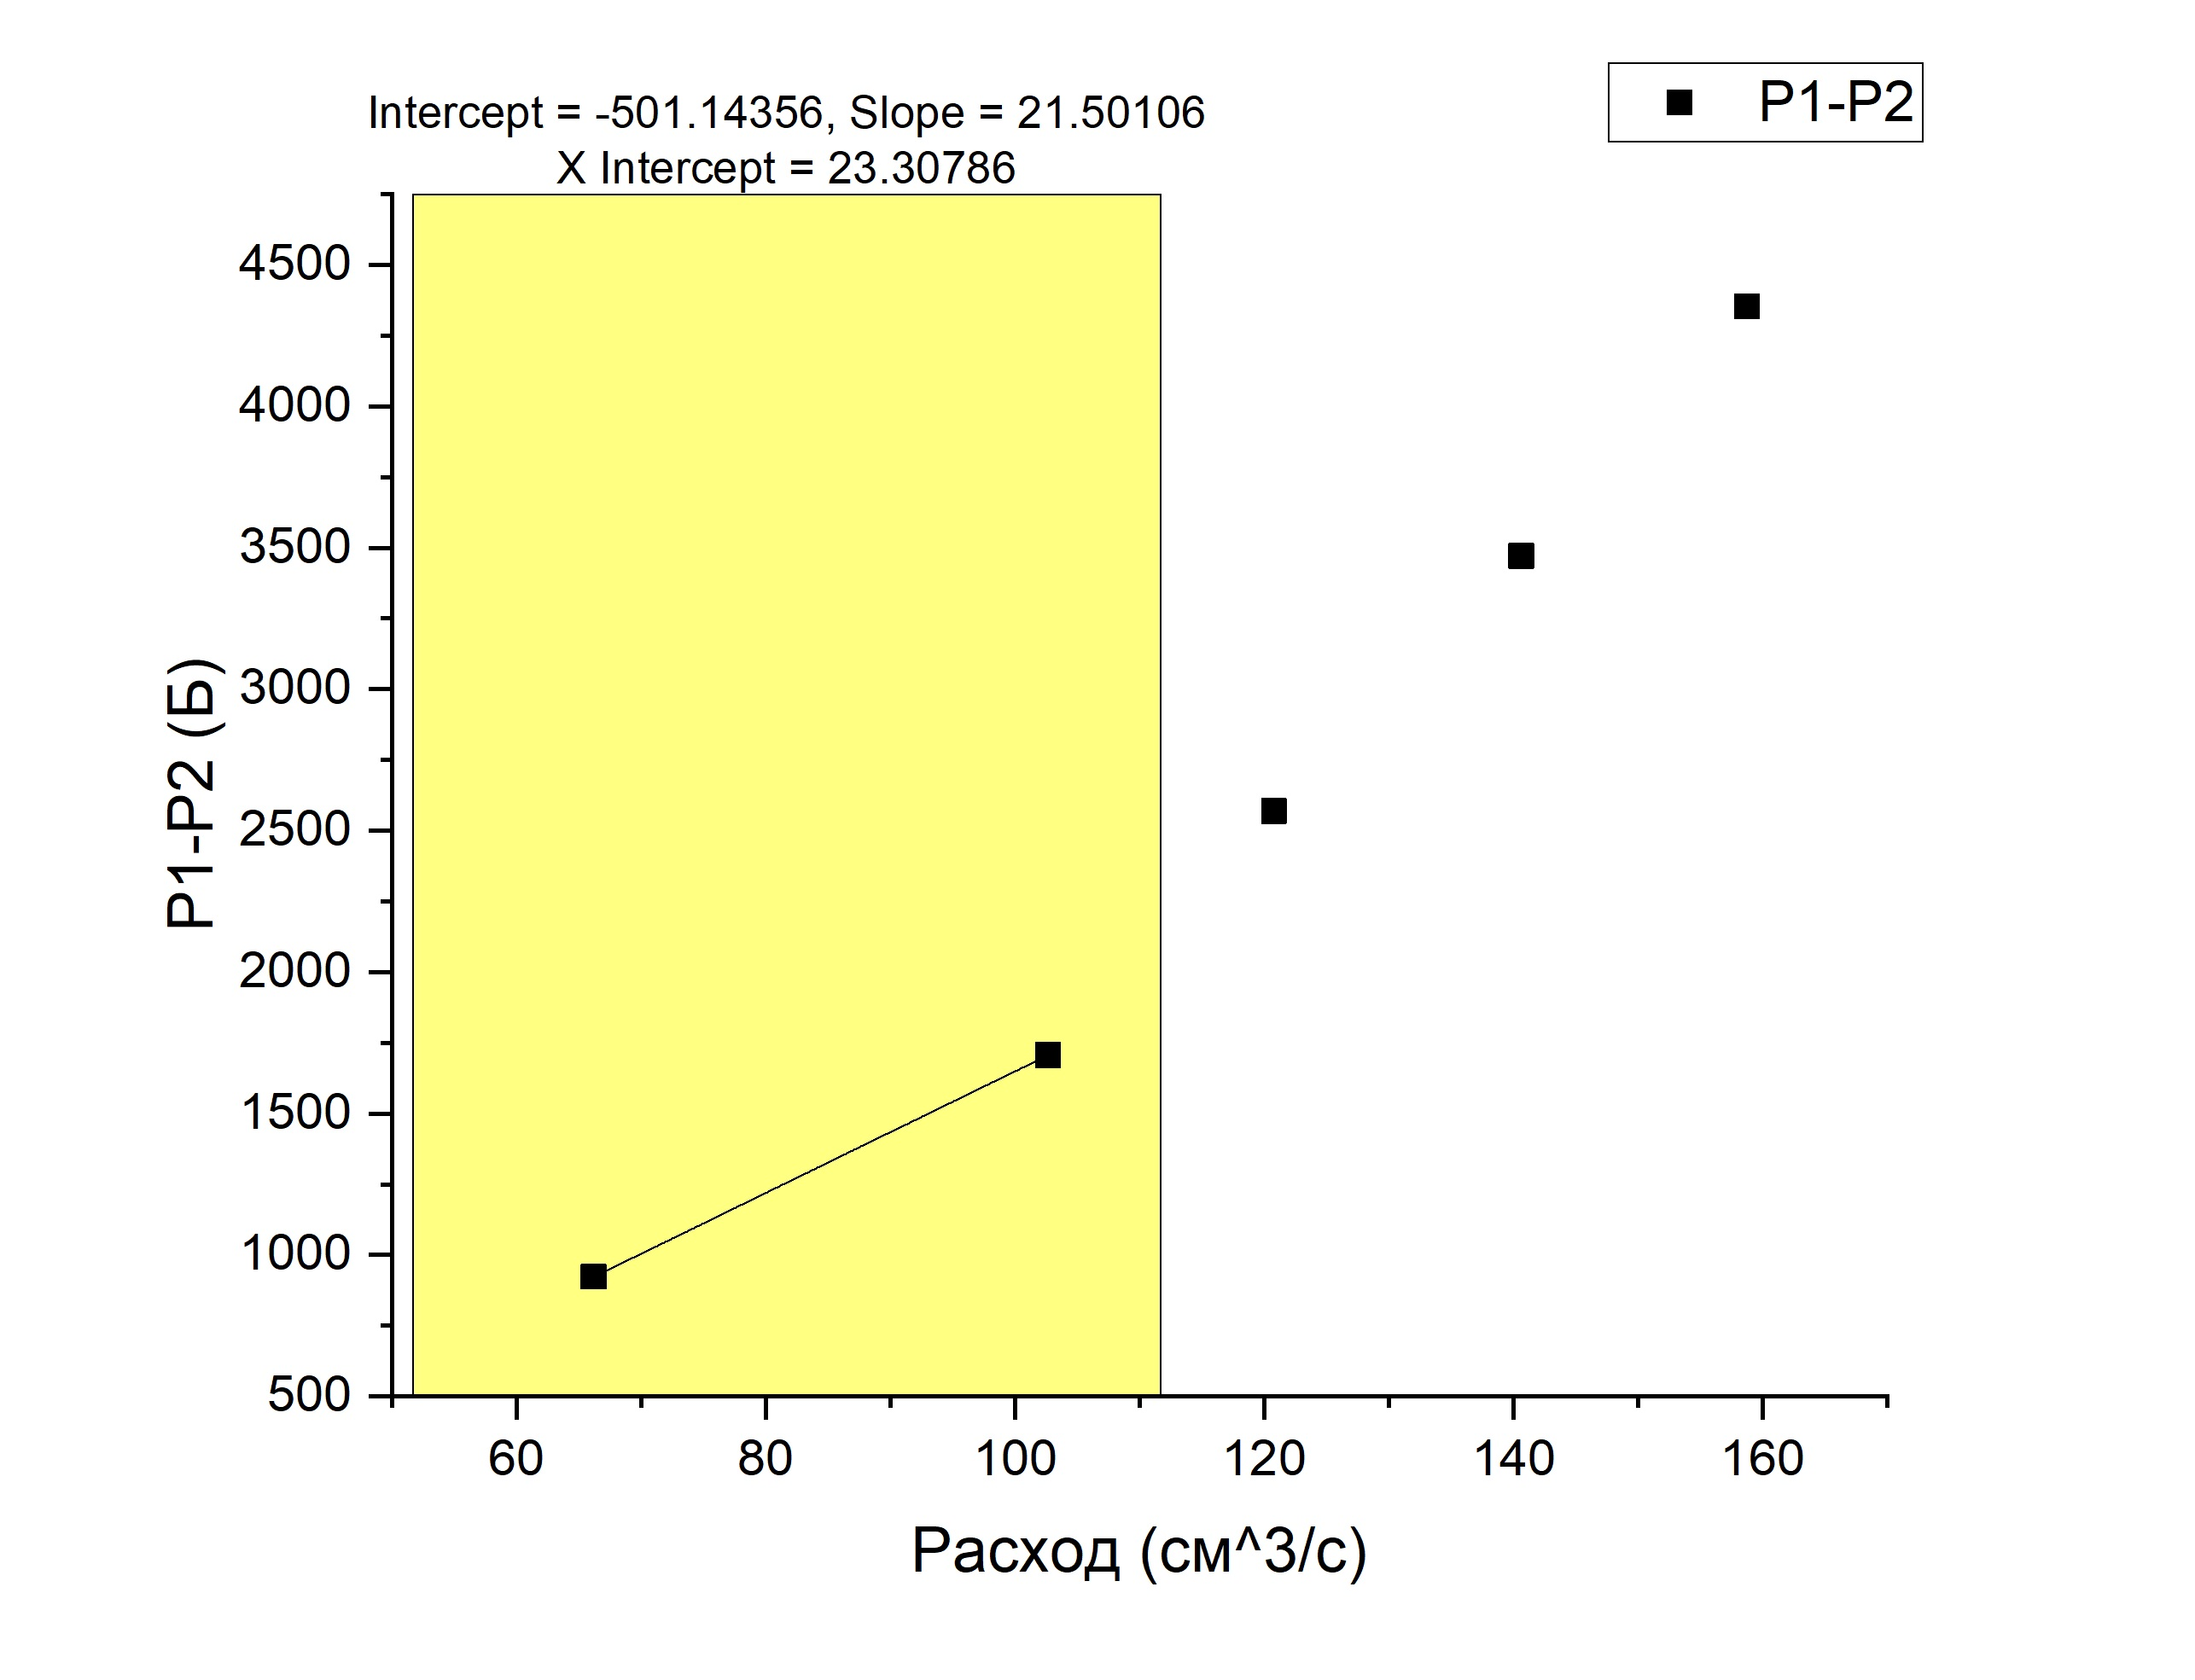
\includegraphics[width=0.80\textwidth]{5.jpg}
	\label{fig:4}
	\caption{Определение $k$ по участку с ламинарным течением}
\end{figure}

Заметим, что на графике \ref{fig:Dp} $k = \frac{8 l \eta}{\pi r^4}$. Значит, 
\begin{equation}
\eta = \frac{\pi r^4 k}{8 l}
\label{eq:Et}
\end{equation}

Определим вязкость.
\begin{table}[htpb]
	\centering
\begin{tabular}{|l|l|l|}
\hline
\textbf{Радиус трубки, см} & \textbf{k} & \textbf{Вязкость, пуаз} \\ \hline
$0.205 \pm 0.0025$               & 21.5       & $29.8*10^{-5}$                \\ \hline
$0.290 \pm 0.0025$               & 11.2       & $62*10^{-5}$               \\ \hline
\end{tabular}
	\caption{Значение $\eta$ для двух трубок}
	\label{tab:Kk}
\end{table}

Можно видеть, что значения вязкости не соответствуют действительности.
\subsection{Выявление зависимости давления от расстояния до входного отверстия}
\begin{figure}[p]
	\centering
		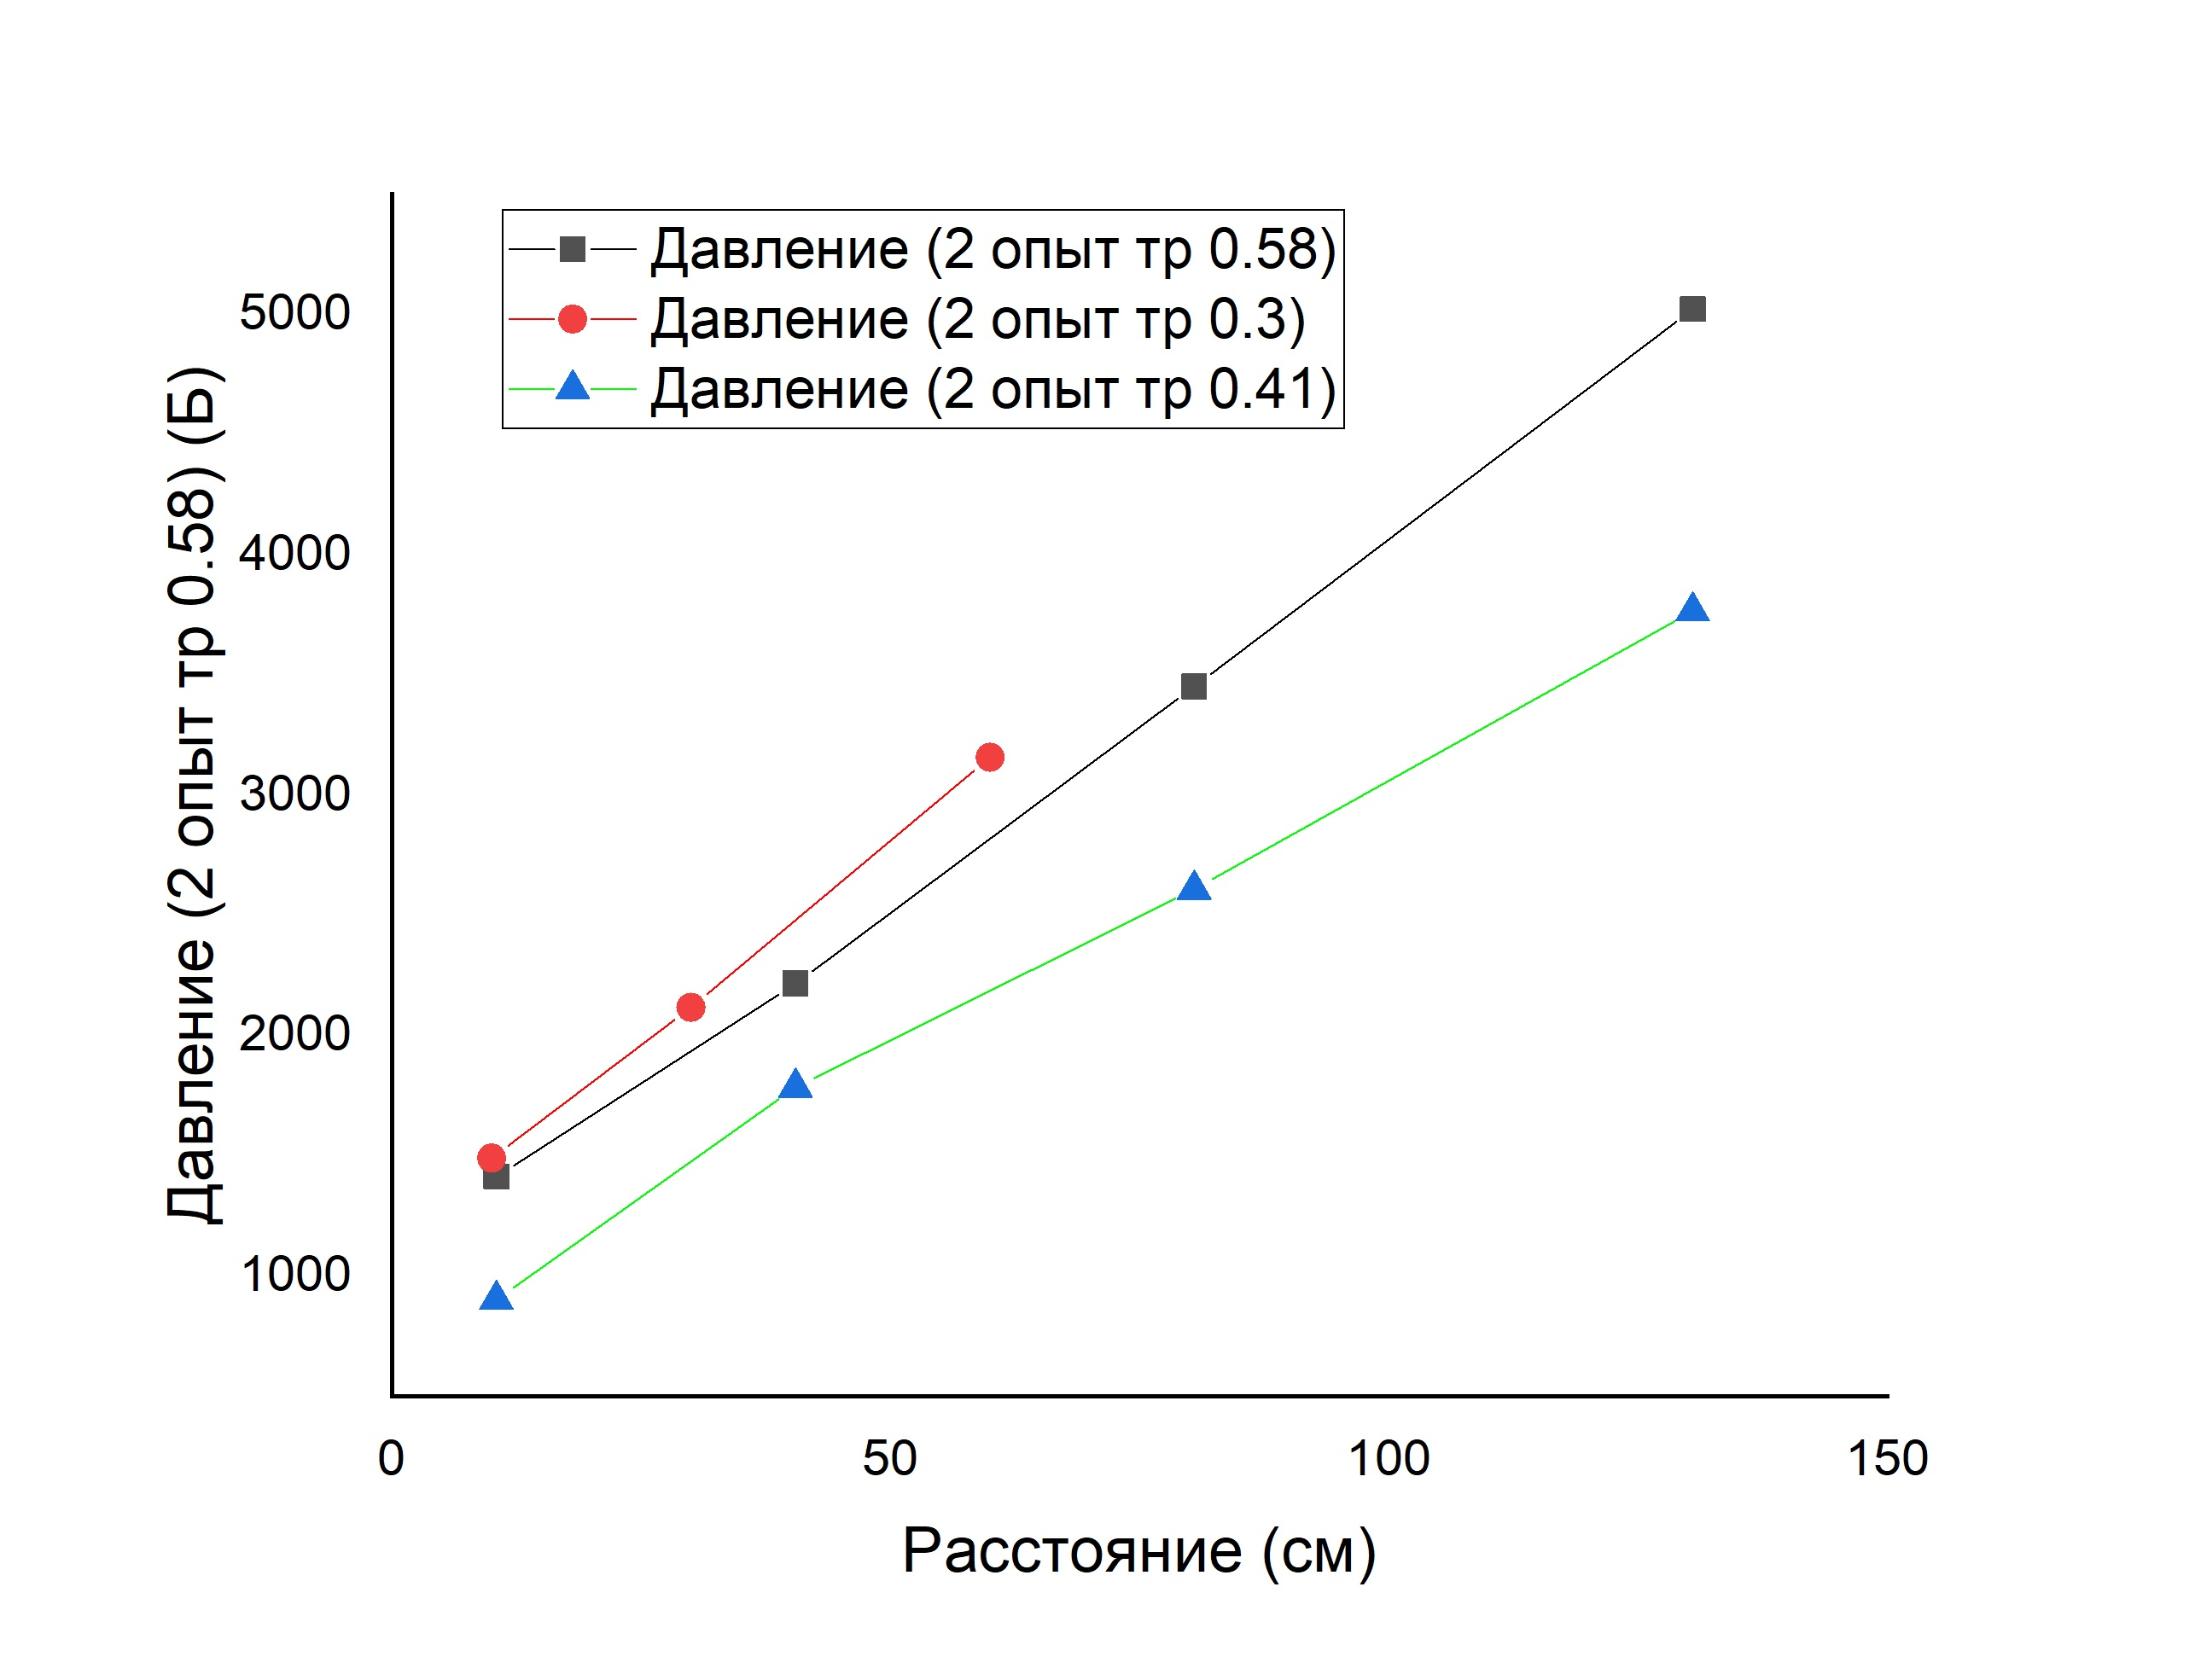
\includegraphics[scale=0.2]{3.jpg}
	\caption{График распределения давления вдоль трубки}
	\label{fig:Pi}
\end{figure}
По графику \ref{fig:Pi} можно видеть, что линейное распределение давления устанавливается на расстоянии, сопоставимом с расчитанным в таблице \ref{tab:Le}.
\section{Вывод}
Так как не было получено достаточно результатов, практически все измерения пришлись на турбулентный поток. Это видно по нелинейности графика $\Delta P = f(Q)$, а также по полученным числам Рейнольдса; таким образом, достоверное вычисление вязкости воздуха по этим данным невозможно.

\end{document}

